\section{\engt{Introduction} \nedt{Introductie}}
\eng{TODO
}

\ned{We maken een lijnvolg robot. Dit is een ingewikkeld project, met veel programmatie. Je kan het op twee manieren aanpakken: de bijgeleverde programma's als gegeven beschouwen en je concentreren op het optimaal maken van de robot. Je kan met de uitleg van deze handleiding de delen van de programma's die meest invloed hebben op het gedrag aanpassen. Kun je al wat meer, probeer dan ook de programma's door te nemen.
}

\subsection{\engt{The components} \nedt{De componenten}}
\eng{We will need the following components: 
\begin{enumerate}
 \item Arduino Uno
 \item Motor Shield 2.5V to max 12V
 \item Echo distance sensor 
 \item line scan sensor
 \item 2 motors (sufficiently powerfull!)
 \item Arduino connector for power to 9V
 \item many wires
 \item mini breadboard
 \item two switches to interrupt the power easily
\end{enumerate}
You will also need a soldering iron, and construction material for the robot. We offer some lasercut designs, but you can use whatever design you like as long as all components fit on it.

For an overview of meaning of the components, see the cheat sheet distributed seperately.
}

\ned{We zullen volgende componenten gebruiken: 
\begin{enumerate}
 \item Arduino Uno
 \item Motor Shield 2.5V tot max 12V
 \item Echo afstandssensor 
 \item line scan sensor
 \item 2 motoren (voldoende krachtig!)
 \item Arduino connector voor stroom naar 9V
 \item veel draden
 \item mini schakelbord
 \item twee schakelaars om de stroom snel te kunnen uitschakelen
\end{enumerate}
Je zal ook een soldeerijzer nodig hebben, en constructiemateriaal voor je robot. We geven een aantal lasercut ontwerpen, maar je kan gelijk welk design gebruiken die je wil, zolang alle componenten er maar op passen.

Voor een overzicht van de betekenis van de componenten, zie het overzicht die je apart gekregen hebt.
}

\subsection{Arduino}
\eng{We will make intensive use of Arduino, so you need to install the \href{http://Arduino.cc}{Arduino software}. Once installed, you can connect the Arduino to your PC via de \textsc{usb} port.  In the programming environment you installed you can write programs, and load those on the Arduino board. They will be executed there as long as the Arduino has power.

}
\ned{We zullen intensief gebruik maken van Arduino, dus moet je de \href{http://Arduino.cc}{Arduino software} installeren op je laptop.
Eenmaal geinstalleerd kun je nu je Arduino koppelen aan je computer via de \textsc{usb} poort. In de programmeeromgeving van Arduino kun je programma's schrijven en die opladen naar de Arduino, waar ze dan uitgevoerd worden zolang er stroom is.
}


\subsection{\engt{Programming with Arduino} \nedt{Programmeren met Arduino}}
\eng{A programming language needs to be understood by a computer. Unfortunately computers are still a little bit dumb, so you are not allowed to make errors! It's like a writing contest in which you need to obtain a 10/10 every time. So take time to learn the form of the language. See the specific sheet 'Programming with Arduino' distributed with this manual.}


\ned{Een programmeertaal moet verstaan worden door een computer. Spijtig genoeg zijn computers nog altijd een beetje dom, dus mag je geen enkele fout maken! Het is zoals een dictee waar je altijd 10/10 moet halen. Neem dus de tijd om de structuur en taal van de Arduino te leren. Zie de blaadjes 'Programmeren met Arduino' die je bij deze gids kan downloaden.}

\section{\engt{Lesson 1: Start! Construction time} \nedt{Les 1: Start! Constuctie}}

\subsection{\engt{Wiring} \nedt{Bedrading}}
\eng{TODO}
\ned{In Figuur \ref{f:wiring} zie je hoe al de componenten aan elkaar moeten verbonden worden. Al deze zaken moeten op je robot passen. De bedrading die je ziet kun je vooraf maken, en dan bepalen hoe je een frame zult maken, en hoe je alles op elkaar zult passen. Het uittesten van alle componenten doen we dan later (al dan niet als het al op een frame zit). 

Voor de AA batterijen die voor Vin zorgen kun je ook krachtige Li-ion batterijen gebruiken. Zorg wel dat je niet meer dan 12V gebruikt. De AA batterijen kunnen veel stroom leveren, wat nodig is voor de motoren. De 9V batterij gebruiken we om de Arduino aan te sturen. Deze 9V batterij kan niet veel stroom leveren, maar de sensoren en de Arduino chip hebben niet veel stroom nodig, dus dat is ok.

Het motor shield die je hebt ziet er niet uit zoals op de figuur. Het concept is hetzelfde evenwel, je hebt 4 schroefconnectors voor de batterijen, 2 voor links, 2 voor rechts. Dan heb je 2 linkse pinnen: PWM en DIR, 2 rechtse pinnen: PWM en DIR. Deze zijn voor de controle van de motoren: hoe snel moeten ze gaan. En dan nog Vin en GND pinnen voor de stroom.

De echo-locator herken je aan de twee ogen. Zet ze niet te hoog zodat je obstakels kunt zien. Er zijn 4 pinnen aan deze sensor: Trig en Echo om de afstand tot een object te bepalen, en dan de VCC en GND voor de stroom, welke 5V \textbf{moet} zijn. 

De lijn scanner heeft 7 pinnen. Voor de stroom opnieuw een VCC en GND, welke opnieuw 5V \textbf{moet} leveren, en dan nog 5 pinnen voor de 5 sensoren die je onderaan ziet. Opgelet, deze sensoren moeten ongeveer 3mm boven de grond hangen. Maak dus een constructie die je toelaat dit wat aan te passen zodat je de juiste hoogte kan instellen.

We gebruiken een mini-schakelbord om correct stroom te leveren. Gebruik een kant voor GND en 5V, en een andere kant voor GND en Vin van de AA batterijen. Schrijf het met alcohol stift op de zijkant, zodat je zeker niet mist. Teveel stroom op de sensoren of de Arduino \textbf{zal} deze kapot maken!
}


\begin{figure}
  \centering
  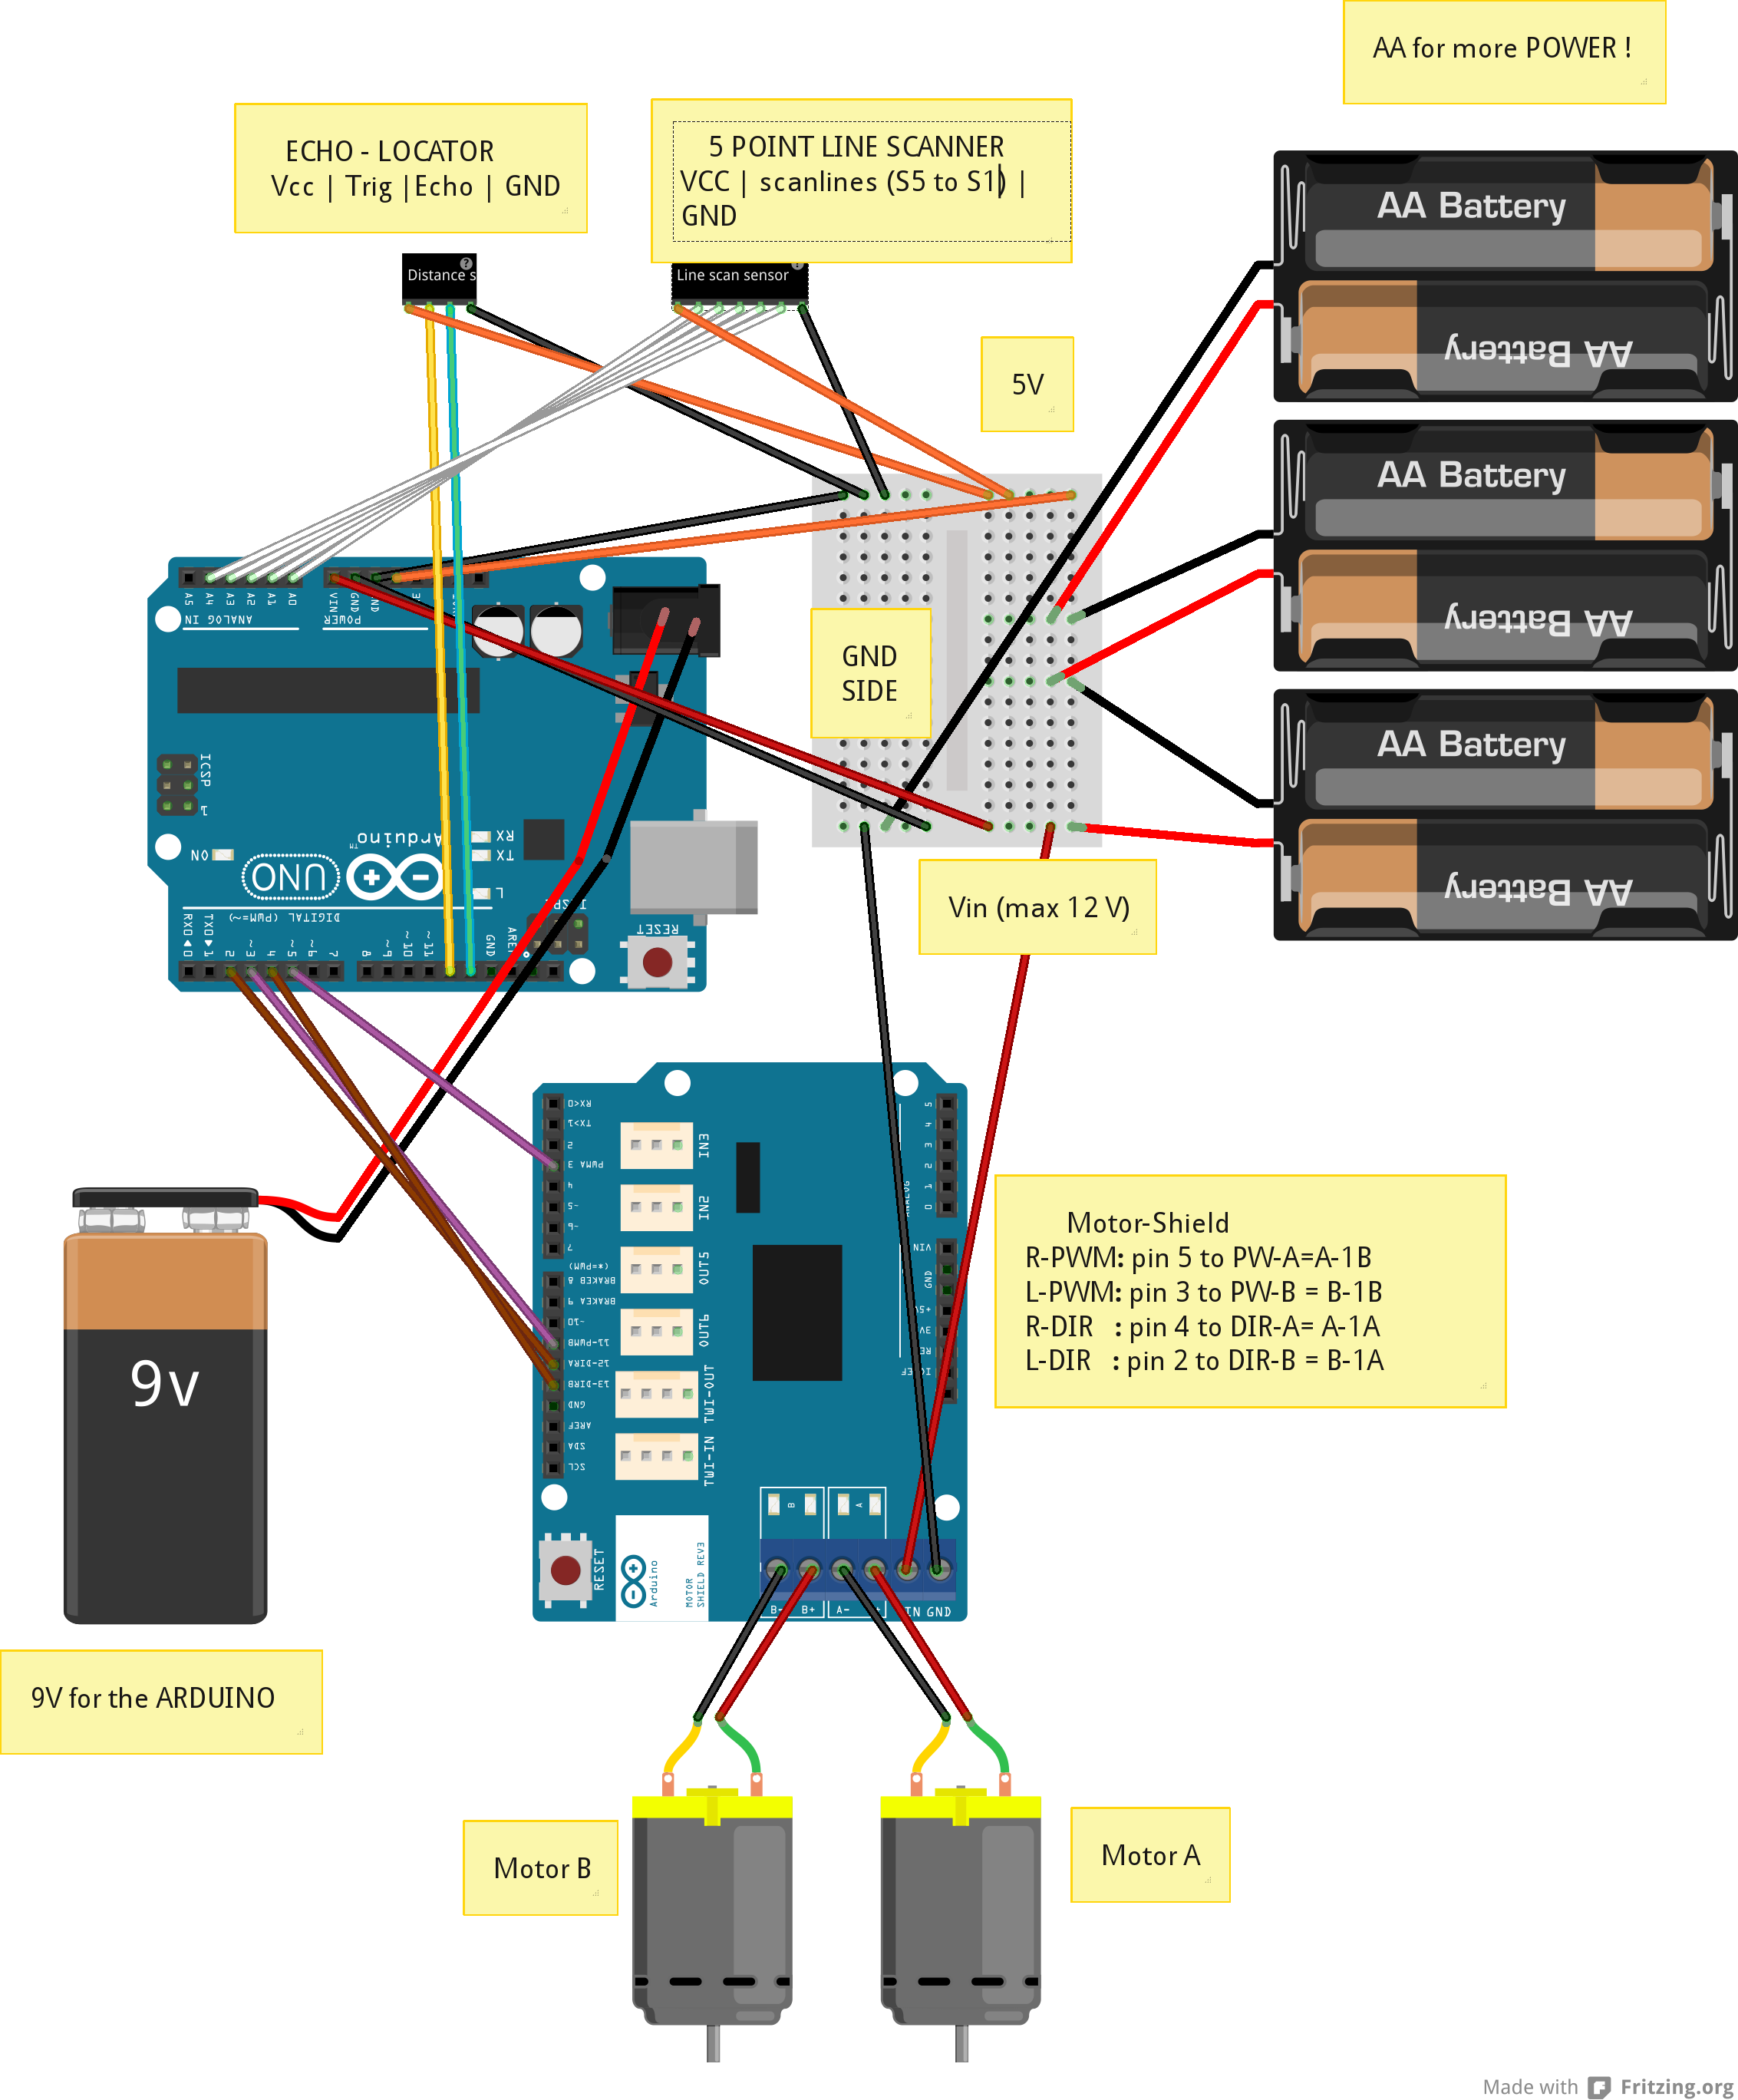
\includegraphics[width=12cm]{img/autorobot_complete_bb.png}
\caption{\engt{The full wiring, all of this must fit on your robot}
\nedt{De volledige bedrading, dit moet helemaal op je robot passen}}
\label{f:wiring}       % Give a unique label
\end{figure}

\subsection{\engt{Construction} \nedt{Constructie}}
\eng{TODO}
\ned{Je weet wat er op je robot moet komen, en kunt dus nu een eigen constructie maken uit materiaal die je hebt liggen. Voorbeelden zie je in Figuur TODO. 

Wil je optimaal werken, dan kun je een frame laten laseren in een fablab in de buurt. Je kan ontwerpfiles vinden in de map \url{https://github.com/ingegno/linefollower1/blob/master/frames/}. Wij zullen frame \textbf{basic} gebruiken. Alle stukken van basic zie je in Figuur \ref{f:frame_basic}, alsook de finale vorm. Voor de stevigheid gebruik je best ook lijm. Dit kan met houtlijm , of, veel gemakkelijker, met een lijmpistool.
}


\begin{figure}[h]
  \centering
  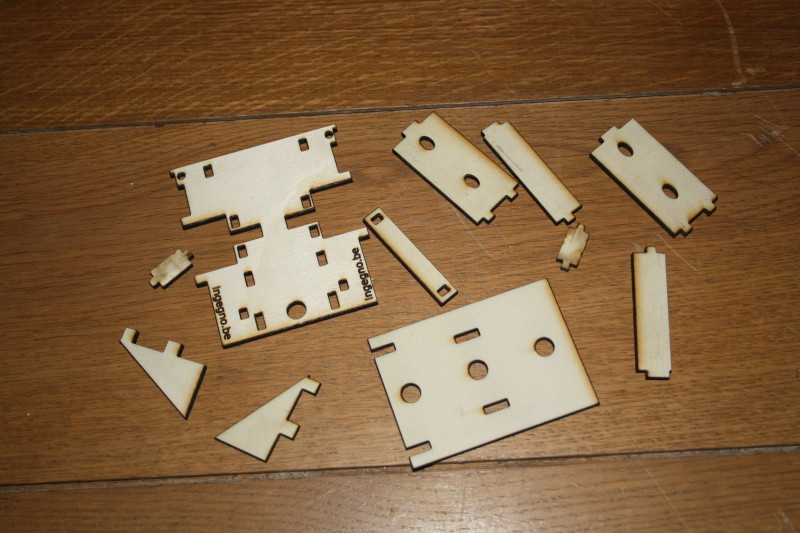
\includegraphics[width=6cm]{pic/20140218T000802005.JPG}
%\rotatebox{-90}{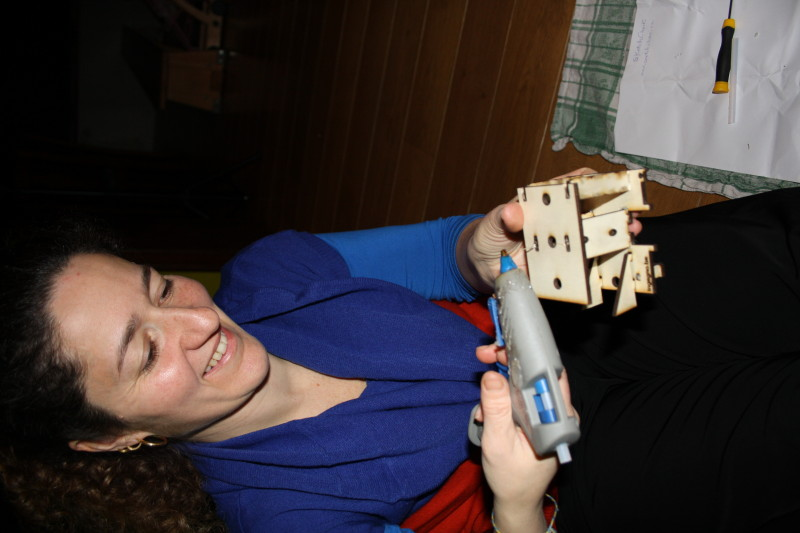
\includegraphics[width=6cm]{pic/20140218T003500016.JPG}} \\
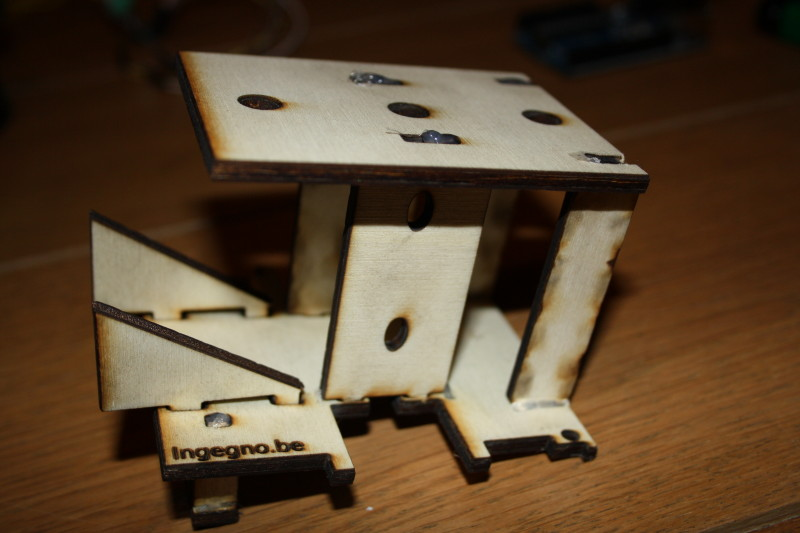
\includegraphics[width=6cm]{pic/20140218T003630017.JPG}
\caption{\engt{Our basic frame, lasercut pieces, glued together form}
\nedt{Ons ``basic'' frame, de gelaserde stukken, en de samengelijmde vorm}}
\label{f:frame_basic}       % Give a unique label
\end{figure}

\eng{TODO}
\ned{Leg nu al je componenten klaar zoals in Figuur \ref{f:components}. We hebben hierbij de motoren reeds bedraad, en aan het motor shield bevestigd (motor A naar A en  motor B naar B). Verder hebben we met twee 3AA batterijhouders, een enkele houder van 9V gemaakt, en er een schakelaar aangehangen. Deze zal de motoren stroom leveren. Voor de Arduino gebruiken we een gewone 9V batterij waar we ook een schakelaar aangehangen hebbben, en een Arduino stroomplug die de Arduino van stroom zal voorzien. Ja, met al deze stukken kunnen we een robot maken, meer is niet nodig! Het wordt wel wat puzzelen om ze allemaal op ons basic frame te krijgen.
}

\begin{figure}[h]
  \centering
  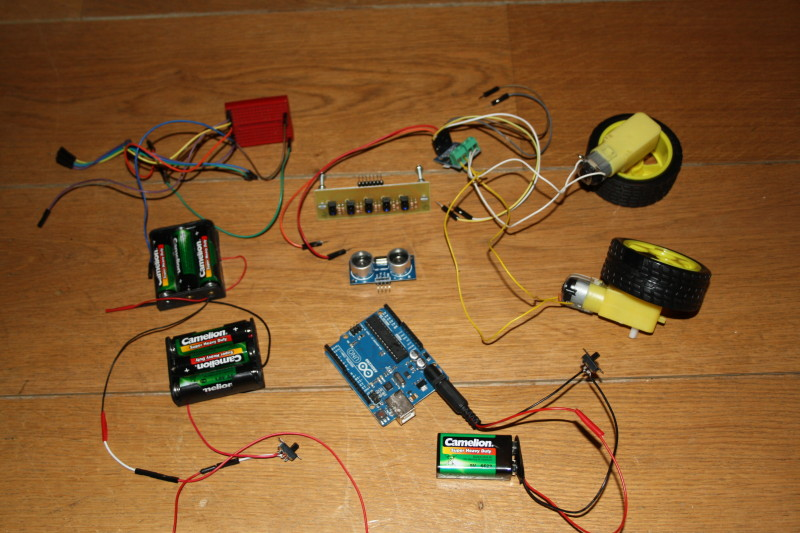
\includegraphics[width=10cm]{pic/20140218T001026006.JPG}
\caption{\engt{All the components}
\nedt{Alle componenten}}
\label{f:components}       % Give a unique label
\end{figure}

\eng{TODO}
\ned{Stap 1 is het vastmaken van de motoren. Het basic frame is zo opgesteld dat deze rechtop staan. Lijm of bindt ze vast aan de rechtopstaande stukken van het frame, zie Figuur \ref{f:fr_motor}. Zorg dat beide motoren op gelijke hoogte staan en nergens tegen slepen. 

Stap 2 is het vastmaken van de lijnscanner. Let goed op wat er op de lijnscanner staat: met de pinnen aan de achterkant staat rechts VCC, en links GND. Daartussen zijn de scanlijnen, welke wij als 0 tot 4 zullen nummeren van rechts tot links, zie Figuur \ref{f:fr_scanlines}. The draden die je gebruikt moeten allen andere kleuren hebben zodat je later goed weet wat wat is. Je laat de draden via een gat onderaan naar boven lopen waar de Arduino zal komen. Met schroeven bevestig je de lijnscanner dan op een hoogte van 3 mm boven de grond als het frame horizontaal staat, zie Figuur \ref{f:fr_scanlines2}.
}


\begin{figure}[h]
  \centering
  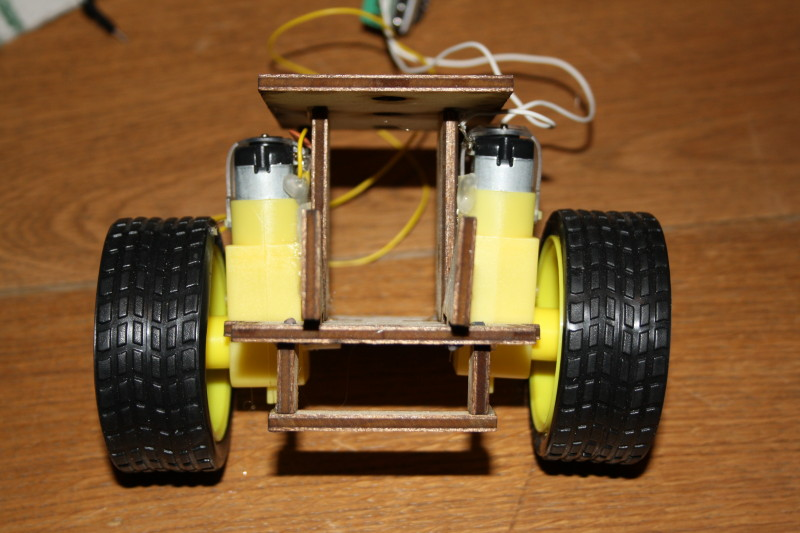
\includegraphics[width=10cm]{pic/20140218T004108018.JPG}
\caption{\engt{The two motors glued to the frame}
\nedt{De twee motoren vastgelijmd op het frame}}
\label{f:fr_motor}       % Give a unique label
\end{figure}

\begin{figure}[h]
  \centering
  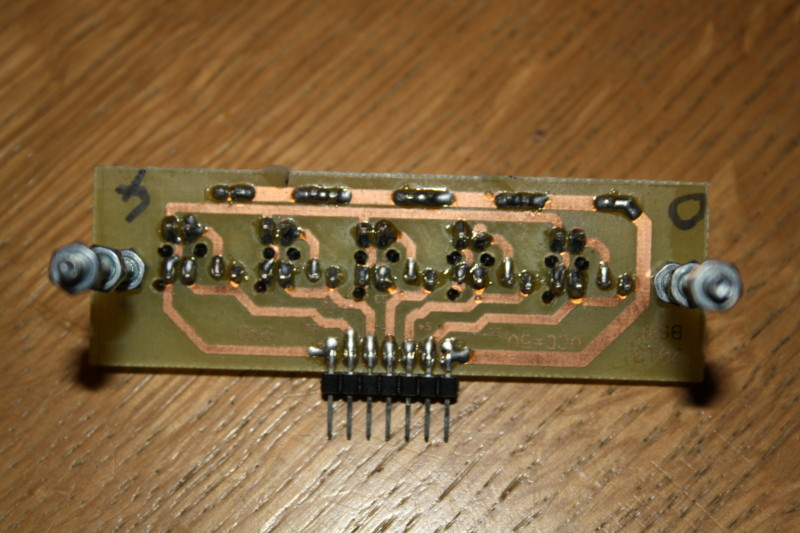
\includegraphics[width=6cm]{pic/20140218T001056008.JPG}
\caption{\engt{The line scanner with 5 scan sensors}
\nedt{De lijnscanner met 5 scan sensoren}}
\label{f:fr_scanlines}       % Give a unique label
\end{figure}

\begin{figure}[h]
  \centering
  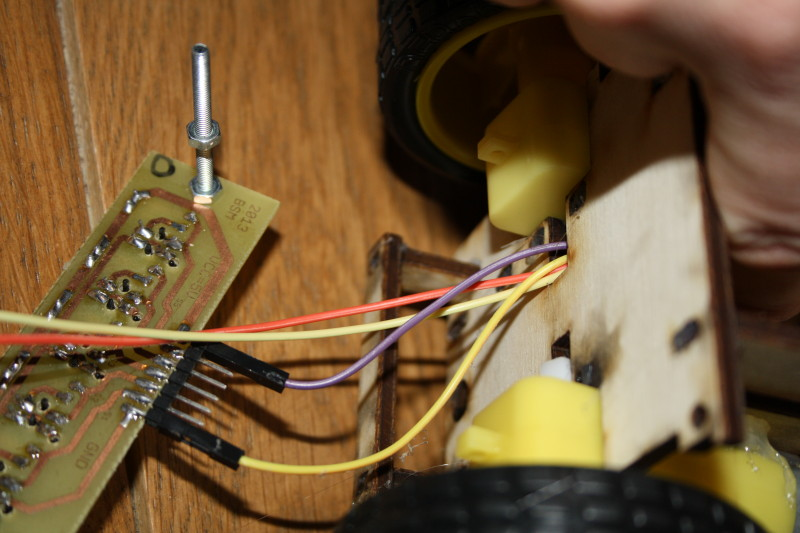
\includegraphics[width=6cm]{pic/20140218T004744019.JPG}
  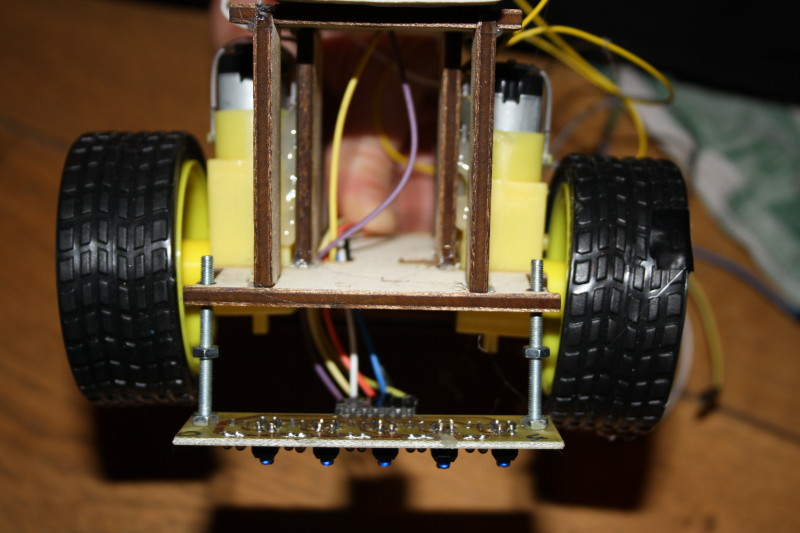
\includegraphics[width=6cm]{pic/20140218T004958020.JPG}
\caption{\engt{Fixing the line scanner to the frame}
\nedt{De lijnscanner vastmaken aan het frame}}
\label{f:fr_scanlines2}       % Give a unique label
\end{figure}


\begin{figure}[h]
  \centering
  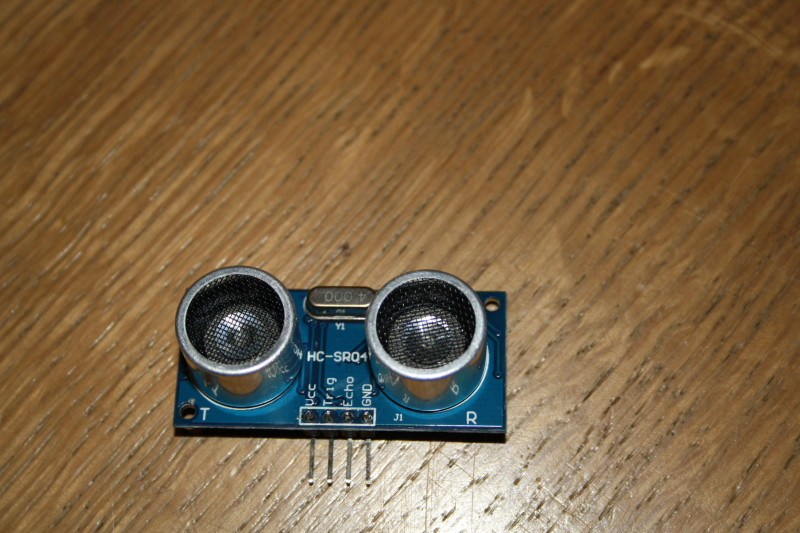
\includegraphics[width=6cm]{pic/20140218T001040007.JPG}
  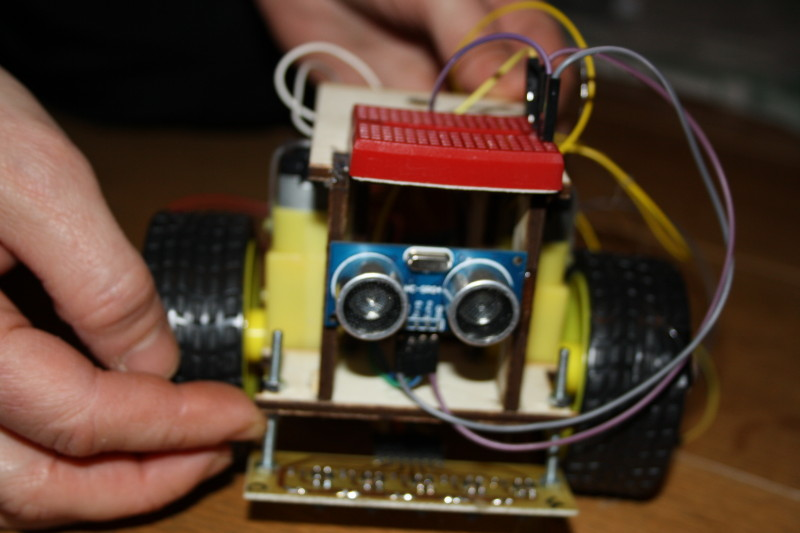
\includegraphics[width=6cm]{pic/20140218T005410022.JPG}
\caption{\engt{The distance scanner are our eyes, and go to the front}
\nedt{De afstandssensor zijn onze ogen, en komen vooraan}}
\label{f:fr_dist}       % Give a unique label
\end{figure}

\eng{TODO}
\ned{Stap 3 is de afstandssensor, die vooraan komt en die vastmaakt op een hoogte waarmee we een blik kunnen zien. De sensor zou precies tussen de voorste pilaren moeten passen, je kan hem eraan binden of vastlijmen. De draden dienen naar boven te lopen, waar we \textbf{VOORAAN} ons mini-schakelbord lijmen. Op het schakelbord gebruiken we een lijn voor Vin, een lijn voor GND van Vin, een lijn voor 5V van de Arduino, en een lijn voor de GND van deze 5V. We gebruiken hiervoor de 4 uiterste lijnen, en schrijven het op het schakelbord in alcoholstift met +, -, Vin en -, zodat we later niet missen. Bevestig de GND en Vcc van de lijnsensor en de afstandssensor tot de - en de + (5V) op het schakelbord. Zie Figuur \ref{f:fr_dist}. Het schakelbord moet boven op het platform vooraan staan omdat we niet willen dat de lijnrobot naar voor kan hellen. De lijnsensoren moeten immers op 3mm boven de grond blijven, dus willen we het zwaarste gewicht (de batterijen) achteraan!

Stap 4 is het plaatsen van onze stroombronnen. Plaats de 9V batterij voor de Arduino tussen de pilaren, en de stroombron Vin voor de motoren (op de foto's de AA batterijen) erachter op de schuine delen. Dit zal ons hoofdgewicht vormen. We willen dat de robot voornamelijk naar achter leunt, maar zorg toch dat dat niet teveel is, zodat de robot niet teveel weegt op het achterste vast punt. De draden van de Vin gaan naar de Vin lijn en de GND lijn op ons schakelbord, zie Figuur \ref{f:fr_power}.
}

\begin{figure}[h]
  \centering
  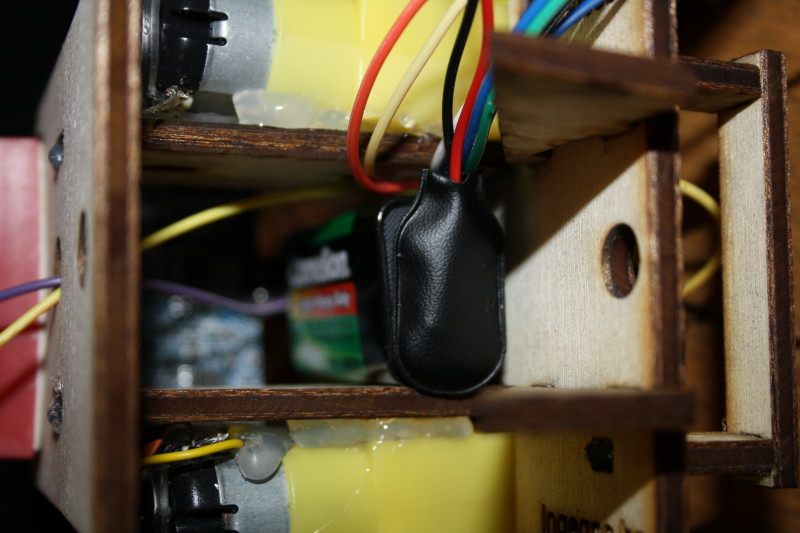
\includegraphics[width=6cm]{pic/20140218T005640023.JPG}
  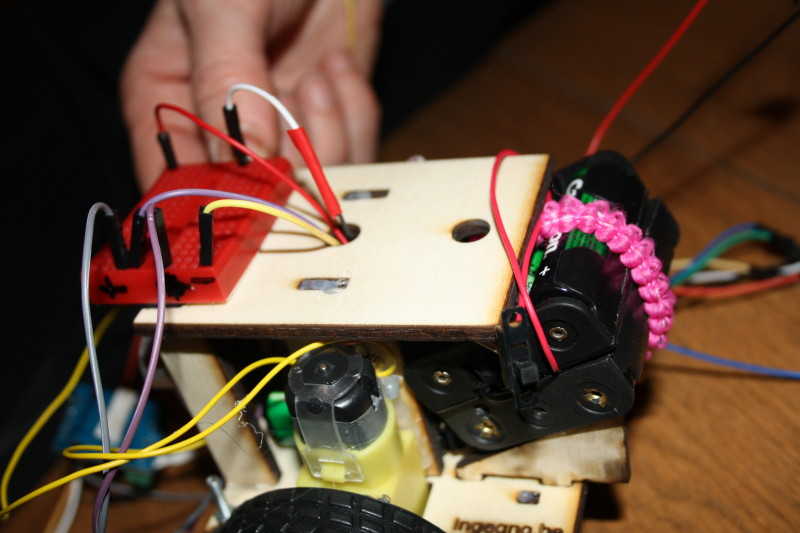
\includegraphics[width=6cm]{pic/20140218T010302024.JPG}
\caption{\engt{The batteries go in the middle and the back}
\nedt{De batterijen gaan tussen de pilaren en langs achter op de spoiler}}
\label{f:fr_power}       % Give a unique label
\end{figure}


\eng{TODO}
\ned{Stap 5 is het plaatsen van de Arduino bovenaan op het frame. Connecteer de rest van de draden voor de lijnsensor en de afstandssensor: de lijnscan outputs gaan naar analoog 0 tot en met 4. Gebruik 0 voor de rechterkant, en 4 voor de linkerkant. Voor de afstandssensor gaat Trig naar pin 12, en echo naar pin 13, zie Figuur \ref{f:wiring} en foto's in Figuur \ref{f:fr_ard}.

Connecteer ok de stroom van de Arduino naar je schakelbord: De eerste GND naar de GND van 5V, en de tweede GND naar de GND van Vin. De Vin pin van de Arduino naar de Vin lijn op het schakelbord, en de 5V pin van de Arduino naar de + (5V) lijn.
}

\begin{figure}[h]
  \centering
  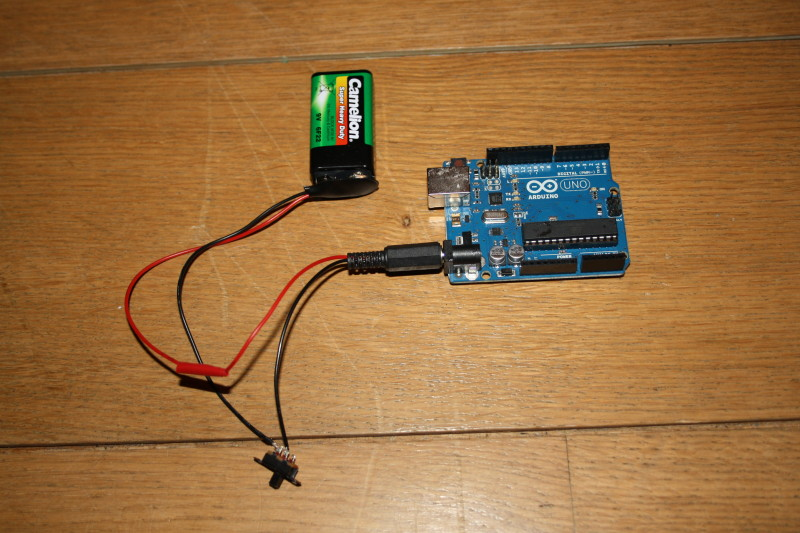
\includegraphics[width=6cm]{pic/20140218T001338012.JPG}
  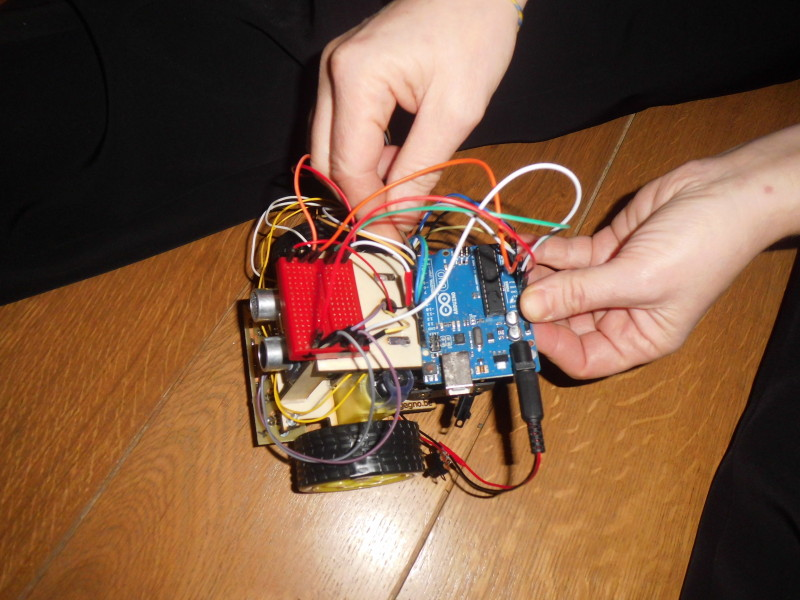
\includegraphics[width=6cm]{pic/Zpart2_20140218T000842031.JPG}
\caption{\engt{Putting the Arduino on the frame}
\nedt{De Arduino komt bovenaan het frame}}
\label{f:fr_ard}       % Give a unique label
\end{figure}

\eng{TODO}
\ned{Stap 6 is het plaatsen van onze laatste component: het motor shield welke al bevestigd was aan de motoren. We stellen voor deze zijwaards op een pilaar te lijmen. De VCC en GND pin van het shield gaan naar de Vin en GND lijn van je schakelbord. Zie Figuur \ref{f:fr_shield}

Met de schakelaars kun je al eens testen: Met Vin zou motor shield LED moeten branden. Afhankelijk van je Arduino zal deze ook al werken en oplichten. Met enkel de Arduino 9V batterij zal enkel de Arduino LED oplichten.

Het motor shield heeft nog 4 extra pinnen: A-1A, A-1B, B-1A en B-1B. A- staat voor motor A, welke voor ons aan de linkerkant is. B- staat voor motor B welke aan de rechterkant is. De 1B pinnen zijn PWM (Pulse Width Modulation) pinnen en dienen dus te lopen naar PWM pinnen op je Arduino welke aangeduid zijn met een golfje: {$\sim$}. We stellen voor dat je doet zoals aangeduid in onze bedrading, Figuur \ref{f:wiring}, dus rechtermotor: B-1A naar pin 2 en B-1B naar pin 3, en voor linkermotor: A-1A naar pin 4 en A-1B naar pin 5.
}


\begin{figure}[h]
  \centering
  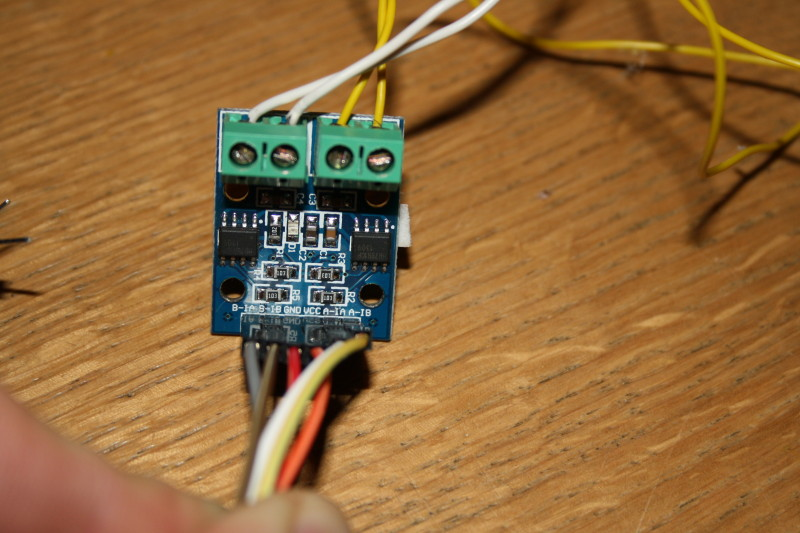
\includegraphics[width=6cm]{pic/20140218T001150010.JPG}
  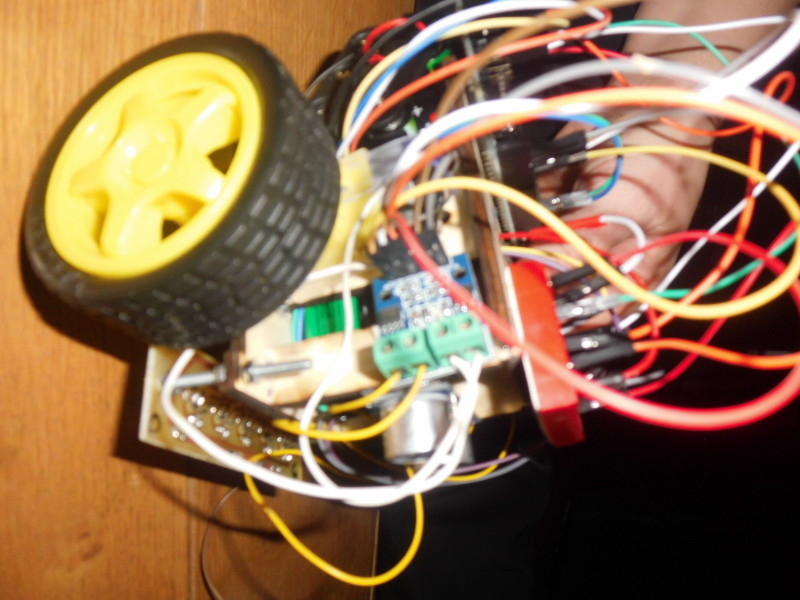
\includegraphics[width=6cm]{pic/Zpart2_20140218T001046033.JPG}
\caption{\engt{The motor shield is attached to the side}
\nedt{Het motor shield komt aan de zijkant}}
\label{f:fr_shield}       % Give a unique label
\end{figure}

\eng{TODO}
\ned{Stap 7 is de balans van de robot. Onderaan aan de achterkant plaats je een wieltje of plak je een kraal zodat de platformen van de robot vlak zijn. Als je een kraal plakt zoals ons, zorg dan wel dat het oppervlak dat sleept op de grond minimaal is, en dat je een materiaal gebruikt dat goed glijdt. Je wil immers niet dat de motoren teveel kracht verliezen om de kraal vooruit te trekken, zeker niet als het meeste gewicht van de batterijen op de kraal leunt.

Als je een wieltje gebruikt dien je te zorgen dat deze zonder probleem kan draaien. Een wiel dat zijwaards sleept als we draaien (bv linkerwiel staat stil als rechter vooruit draait) zal immers meer problemen geven dan een kraal!
}

\eng{TODO}
\ned{Stap 8 is algemene schoonmaak: ziet het er goed uit? Gebruik lintjes om de kabels ordentelijk weg te moffelen. Gebruik wat versiering om je robot er geduchter te laten uitzien! Wat je ook doet, stuur ons een mailtje met je kunstwerk!
}

\newpage
\section{\engt{Lesson 2: Drive!} \nedt{Les 2: Rijden maar}}
\eng{TODO}
\ned{We beginnen met de motoren uittesten. Is links echt links? Is vooruit echt vooruit? Laad de code uit Code \ref{c:l1_motor} op je Arduino, en volg mee in de code of robot doet wat het programma opgeeft. 

Als het fout gaat dien je de connecties op je motor shield aan te passen. Links met rechts wisselen is A en B omwisselen. Vooruit in achteruit veranderen op A is de draden van A omwisselen. Idem voor B vooruit in achteruit wijzigen.

Hoe werkt het programma? Wel, we definieren eerst op welke pinnen onze motors zitten. De Dir pinnen geven de richting aan: vooruit of achteruit. Als je het goed deed zou \ardo{LOW} moeten vooruit zijn, en \ardo{HIGH} achteruit. De Dir pinnen zetten is evenwel niet genoeg. Je moet ook doorgeven via PWM pinnen hoeveel kracht de wielen moeten hebben, dus hoe snel ze moeten draaien. Voor \ardo{LOW} is dat een waarde van 0 tot 255, met 0 stilstaan en 255 de maximale snelheid. Voor \ardo{HIGH} is het omgekeerd: een waarde van 255 tot 0 met 255 stilstaan, en 0 de maximale snelheid.

Om eenvoudig te werken schrijven we een functie \ardo{void motor_drive (int right_speed, int left_speed)}. Deze functie krijgt als parameter de snelheid mee waarmee we willen dat de motor werkt. Dit dienen waarden tussen -255 en 255 te zijn. Negatieve getallen interpreteren we als achteruit, positieve als vooruit.

Het is belangrijk dat je de calibratiewaarden correct zet voor jou robot. Wat is de hoogste snelheid die je wil? Wat is de waarde van PWM die zorgt dat motor niet langer beweegt voor jou? Indien je robot niet op een rechte lijn rijdt bij vooruit, dien je ook links en rechts te corrigeren om dit juist te krijgen. Dit zijn \ardo{calib_speed_corrR} en \ardo{calib_speed_corrL} in de Code.
}

\begin{code}\label{c:l1_motor}
 \ \newline
\inputardfull{\string"../sketches/calib_motors_forward/calib_motors_forward.ino\string"}
\end{code}

\eng{TODO}
\ned{Als de vorige code goed werkte, gaan we over op de volgende test: rond de as draaien. De aangepaste \ardo{loop} functie staat in Code \ref{c:l2_motor}. Het enige dat verschillend is is dat we nu ook negatieve waarden gebruiken om roteren rond de as te verkrijgen. We draaien eerst anti-klokwijs, en dan volgens de klok. Telkens voor 3 seconden. 
}

\begin{code}\label{c:l2_motor}
 \ \newline
\inputard{\string"../sketches/calib_motors_rotate_axis/calib_motors_rotate_axis.ino\string"}{37}{54}
\end{code}


\engo{\begin{doE}
     With the two previous codes you have everything to write a predetermined circuit. So, decide on the circuit you want your robot to follow, and change the \ardo{loop} function of the previous code so that your robot performs the circuit you decided.
     \end{doE}
}
\nedo{\begin{doN}
     Met de twee vorige codes heb je alles om je eigen voorgeprogrammeerd parcours af te leggen. Beslis een parcours die je wil dat je robot aflegd, en wijzig de \ardo{loop} functie van je vorige code om dit parcours te verkrijgen. 
     \end{doN}
}


\section{\engt{Lesson 3: Light sensor setup} \nedt{Les 3: een lichtsensor gebruiken}}
\eng{TODO}.
\ned{De tweede stap is het monteren van de lichtsensor. De lichtsensor kan kleuren detecteren onder de sensor.}


\begin{code}\label{c:l2_c}
 \ \newline
\inputardfull{\string"../sketches/calib_light_sensor_setpoint_line_follow/calib_light_sensor_setpoint_line_follow.ino\string"}
\end{code}


\section{\engt{Lesson 4: Follow a line} \nedt{Les 4: Een lijn volgen}}
\eng{TODO}.
\ned{Met motoren en de lichtsensor kunnen we een lijn volgen
}

\subsection{\engt{Basic version: move to midline} \nedt{Basisversie: beweeg naar een middellijn}}

\eng{TODO}
\ned{Ons basisalgoritme werkt op basis van volgend principe: 
\begin{enumerate}
 \item We lezen de lichtsensor in. We bepalen het middelpunt zoals in les 2: gewogen gemiddelde van de 5 sensoren. Gezien deze van 0 tot en met 4 lopen, zou het midden 2 moeten zijn. 
 \item De fout is het verschil van het gemeten middelpunt en het gewenste middelpunt, maal 1000. We willen deze fout zo klein mogelijk houden.
 \item Op basis van de fout passen we de snelheid van de motoren aan in de functie \ardo{calc\_turn}. De snelheid van de motoren is een getal tussen \ardo{min\_speed} en \ardo{max\_speed}, waarbij de eerste de waarde van PWM is die overeenkomt met stilstand (typisch 0), en \ardo{max\_speed} de maximum snelheid die je wil (typisch 180 tot 254). We corrigeren de snelheid van de linker of rechtermotor dus met
$$\frac{\mathrm{fout}}{\mathrm{max\_fout}} \times ( \mathrm{max\_speed} - \mathrm{min\_speed} ).
$$
 \item De correctie wordt verminderd van de snelheid van het wiel dat rotatie in de correcte richting veroorzaakt.
\end{enumerate}
}

\begin{code}\label{c:l3_c}
 \ \newline
\inputardfull{\string"../sketches/calib_forward_line_follow/calib_forward_line_follow.ino\string"}
\end{code}

\subsection{\engt{Extended version: types of lines} \nedt{Uitgebreide versie: type lijnen}}

\eng{TODO}
\ned{Ons basisalgoritme werkt op eenvoudige, traag draaiende lijnen. Zodra het wat sneller gaat, of bij scherpe bochten gaat het mis. Er kunnen verschillende manieren bedacht worden om dit op te lossen. 

Laat ons de volgende aanpak kiezen: we bepalen een type lijn. In plaats van enkel in \ardo{sensors_read()} te bepalen of we een lijn zien of niet, onderscheiden we volgende gevallen, die we als geheel getal (integer, dus int) teruggeven:
\begin{enumerate}
 \item \ardo{#define LS\_UNKNOWN    0 // we kunnen niet bepalen wat we zien}
 \item \ardo{#define LS\_BLACKLINE  1 // een zwarte lijn}
 \item \ardo{#define LS\_BLACKFIELD 2 // een zwart veld}
 \item \ardo{#define LS\_WHITEFIELD 3 // een wit veld}
 \item \ardo{#define LS\_BLACKLEFT  4 // zwart afbuigend naar links}
 \item \ardo{#define LS\_BLACKRIGHT 5 // zwart afbuigend naar rechts}
 \item \ardo{#define LS\_BLACKSPLIT 6 // zwart links en rechts, niet midden}
\end{enumerate}
Pas de functie \ardo{sensors_read()} aan om op basis van de gemeten waarden te bepalen wat er gebeurt. Pas dan de \ardo{loop()} functie aan met een switch op basis van het resultaat: \ardo{switch (sensors_read())}. Voor \ardo{LS\_BLACKLINE} is het zoals in de basisversie, maar doe nu andere bewegingen in de andere gevallen.

Onze aanpak kun je vinden op \url{https://github.com/ingegno/linefollower1/blob/master/sketches/calib_forward_line_follow_extend/calib_forward_line_follow_extend.ino}.
}

\section{\engt{Lesson 5: Distance to an object} \nedt{Les 5: Afstand tot een object.}}
\eng{TODO}

\ned{We plaatsen nu ogen op onze robot. De ogen zijn in werkelijkheid ultrasone sensoren, die de afstand bepalen tot objecten voor zich op dezelfde wijze als vleermuizen dat doen. 

De code kan gevonden worden in \ref{c:l4_c}.
}

\begin{code}\label{c:l4_c}
 \ \newline
\inputardfull{\string"../sketches/calib_distance_sensor/calib_distance_sensor.ino\string"}
\end{code}



\section{\engt{Lesson 6: Search and push object} \nedt{Les 6: Zoek en duw object.}}
\eng{TODO}

\ned{Integreer nu de code uit les 4 in de code van les 3. Zorg dat de robot niet rijdt als niet op een zwarte lijn. We zullen nu het volgende probleem beschouwen: Veronderstel dat je op een zwarte lijn was, en op een wit veld komt. Verifieer of dat waar is (dus je echt op een zwarte lijn was). Zoek op het witte veld een object, en duw het uit het veld.

In de code zullwen we dus in het geval van \ardo{case LS\_WHITEFIELD:}, code uitvoeren om dit te bereiken. Gezien onze code in de loop de lijn probeert te lezen, en we nu iets anders moeten doen dat vastligt (zoeken, bewegen naar, en dan wegduwen), doen we alles zonder gebruik te maken van de Arduino loop. Met andere woorden, we gebruiken de \ardo{while (allesok)} constructie om acties te laten voortduren tot we een gewenst resultaat hebben.

De veranderingen kunnen gevonden worden in \ref{c:l5_c}.
}

\begin{code}\label{c:l5_c}
 \ \newline
\inputard{\string"../sketches/calib_search_push_object/calib_search_push_object.ino\string"}{59}{75}
 \ \newline
\inputard{\string"../sketches/calib_search_push_object/calib_search_push_object.ino\string"}{163}{321}
\end{code}
